\section[Candidatos fraccionarios no Chua]{Sistemas fraccionarios no Chua: realización y dinámica}
\label{part:nonchua}

\section{Sistemas considerados}

Estudiamos dos problemas relacionados: representar exactamente el campo
mediante canales estáticos y determinar qué condiciones iniciales permiten
alcanzar sus conjuntos atractivos. Desarrollamos primero la representación,
los equilibrios y la estabilidad local. La cota de absorción de Lorenz
controla el crecimiento de las soluciones; la identificación de un atractor
requiere, además, estudiar el destino de las semillas y sus cuencas.

Dos sistemas fraccionarios no Chua están vinculados de forma explícita con
atractores ocultos en la bibliografía analizada: el Lorenz generalizado y el
sistema de Rabinovich--Fabrikant (RF), ambos estudiados por
Danca~\cite{Danca2017}. El Lorenz estándar y otra
parametrización de RF sirven como referencias para exponentes de Lyapunov, junto con
los sistemas jerk exponencial, financiero y \emph{four-wing} de
Fischer et al.~\cite{fischer2020}. Ambos conjuntos de casos tienen alcances
distintos y se presentan por separado.

\begin{table}[ht]
\centering
\small
\caption{Sistemas y alcance del análisis.}
\begin{tabularx}{\linewidth}{>{\raggedright\arraybackslash}p{0.23\linewidth}
>{\raggedright\arraybackslash}p{0.19\linewidth}X}
\toprule
Caso & Análisis & Resultado y límite\\
\midrule
Lorenz generalizado, \(q=0.995\) & Algebraico &
Realización multicanal, tres equilibrios y espectros; existencia global y
absorción de reinicios. La dinámica del candidato y su cuenca se conocen
por la referencia bibliográfica.\\
Rabinovich--Fabrikant, \(q=0.998\) & Algebraico &
Realización multicanal, cinco equilibrios, espectros y radios bibliográficos
de vecindad. Falta reproducir el atractor y su cuenca.\\
Lorenz estándar, RF \(b=0.98\), jerk, financiero y four-wing & diagnóstico
numérico & Ecuaciones, parámetros, análisis local, protocolo de integración y
comparaciones de exponentes de Lyapunov. Estas pruebas no incluyeron una
búsqueda de cuencas ni certifican ocultedad.\\
Genesio--Tesi, jerk hiperbólico y otras familias escalares & Algebraico &
Realizaciones escalares y cierres armónicos; falta completar la localización
y la evaluación dinámica.\\
\bottomrule
\end{tabularx}
\end{table}

Las realizaciones de Genesio--Tesi y de los sistemas memristivos proporcionan
problemas de localización. Los cinco sistemas de referencia dinámica permiten
comparar diagnósticos de Lyapunov, pero carecen de continuación desde una
semilla y de sondeos de vecindad. Sus exponentes no establecen ocultedad.

\section[Marco común de realización]{Marco común de realización y localización}

\subsection{Dinámica de Caputo y transferencia fraccionaria}

Para \(0<q<1\) y un estado absolutamente continuo en cada intervalo de
integración, la derivada de Caputo con terminal inferior \(t_0\) se escribe
\begin{equation}
 {}^{\mathrm C}D_{t_0}^{q}x(t)
 =\frac{1}{\Gamma(1-q)}
 \int_{t_0}^{t}(t-\tau)^{-q}x'(\tau)\,d\tau .
 \label{nc:eq:caputo}
\end{equation}
La ecuación autónoma
\begin{equation}
 {}^{\mathrm C}D_{t_0}^{q}x(t)=F(x(t)),\qquad x(t_0)=x_0,
 \label{nc:eq:ivp}
\end{equation}
es equivalente a la ecuación integral de Volterra
\begin{equation}
 x(t)=x_0+\frac{1}{\Gamma(q)}
 \int_{t_0}^{t}(t-\tau)^{q-1}F(x(\tau))\,d\tau .
 \label{nc:eq:volterra}
\end{equation}
La historia desde \(t_0\) es parte del problema; no puede reiniciarse durante
una continuación sin declarar que se ha definido un problema diferente.

Para el bloque lineal
\begin{equation}
 {}^{\mathrm C}D_{t_0}^{q}x=Ax+Bu,
 \qquad y=Cx,
 \label{nc:eq:linear-block}
\end{equation}
introducimos el tiempo transcurrido \(u=t-t_0\) y definimos
\(X(s)=\int_0^\infty e^{-su}x(t_0+u)\,du\). En el semiplano donde
existen las transformadas, la identidad de Caputo da
\begin{equation}
 \mathcal L\{{}^{\mathrm C}D_{t_0}^{q}x\}(s)
 =s^qX(s)-s^{q-1}x(t_0).
\end{equation}
Al transformar la ecuación lineal resulta
\[
 (s^qI-A)X(s)=s^{q-1}x(t_0)+BU(s).
\]
Con estado inicial nulo y \(s^q\notin\operatorname{spec}(A)\),
la transferencia entrada--salida es
\begin{equation}
 W_q(s)=C(s^qI-A)^{-1}B.
 \label{nc:eq:transfer-general}
\end{equation}
Se usa la rama principal. En el predictor armónico,
\begin{equation}
 (\ii k\omega)^q=(k\omega)^q
 \exp\!\left(\ii\frac{q\pi}{2}\right),\qquad k>0.
 \label{nc:eq:principal-branch}
\end{equation}
Esta sustitución produce un problema algebraico estacionario; no afirma la
existencia de una órbita periódica exacta del PVI causal de Caputo.

\subsection{Realización de Lur'e multicanal}

Los dos candidatos no son escalares en su no linealidad. Se usa la forma exacta
\begin{equation}
 {}^{\mathrm C}D_{t_0}^{q}x=Ax+B\Phi(Cx),
 \qquad x\in\RR^n,
 \label{nc:eq:mimo-lure}
\end{equation}
con \(\Phi:\RR^p\to\RR^m\) estática. La identidad que debe comprobarse es
\begin{equation}
 Ax+B\Phi(Cx)-F(x)\equiv0.
 \label{nc:eq:lure-residual}
\end{equation}
No basta que las expresiones coincidan en una trayectoria o en un equilibrio.

Sea \(\bar y=C\bar x\) un sesgo y
\begin{equation}
 K=D\Phi(\bar y)\in\RR^{m\times p}.
\end{equation}
La ecuación de cierre linealizada del primer armónico es
\begin{equation}
 \det\!\left[I_p-W_q(\ii\omega)K\right]=0.
 \label{nc:eq:det-closure}
\end{equation}
Para amplitud finita, \(K\) se sustituye por los coeficientes de Fourier
exactos de la no linealidad.

\subsection{Coeficientes exactos y balance multiharmónico}

Se adopta la convención compleja
\begin{equation}
 x(\theta)=\sum_{k=-H}^{H}X_k e^{\ii k\theta},
 \qquad X_{-k}=\overline{X_k},\qquad X_0\in\RR^n,
 \label{nc:eq:fourier-state}
\end{equation}
con \(\theta=\omega t\). Si \(u\) y \(v\) tienen coeficientes \(U_k,V_k\),
la multiplicación no se aproxima: sus coeficientes son la convolución
\begin{equation}
 \widehat{(uv)}_k=\sum_{m\in\mathbb Z}U_mV_{k-m}.
 \label{nc:eq:conv2}
\end{equation}
Para un producto triple,
\begin{equation}
 \widehat{(uvw)}_k
 =\sum_{m\in\mathbb Z}\sum_{n\in\mathbb Z}
 U_mV_nW_{k-m-n}.
 \label{nc:eq:conv3}
\end{equation}
En una truncación se toma \(U_k=0\) para \(|k|>H\). Esto calcula exactamente
los coeficientes retenidos de la señal truncada; la omisión de armónicos altos
se controla aumentando \(H\).

Si \(\widehat\Phi_k\) denota el coeficiente \(k\) de \(\Phi(Cx(\theta))\), el
sistema completo de balance es
\begin{align}
 AX_0+B\widehat\Phi_0&=0,
 \label{nc:eq:hb0}\\
 \left[(\ii k\omega)^qI-A\right]X_k-B\widehat\Phi_k&=0,
 \qquad k=1,\ldots,H.
 \label{nc:eq:hbk}
\end{align}
Las incógnitas son \(X_0,X_1,\ldots,X_H,\omega\), junto con una condición de
fase, por ejemplo
\begin{equation}
 \operatorname{Im}(e_j\trans X_1)=0,\qquad
 \operatorname{Re}(e_j\trans X_1)>0.
 \label{nc:eq:phase-condition}
\end{equation}
Una familia de estados iniciales se reconstruye mediante
\begin{equation}
 x_{\mathrm{sem}}(\varphi)=X_0+
 2\operatorname{Re}\sum_{k=1}^{H}X_ke^{\ii k\varphi}.
 \label{nc:eq:seed-reconstruction}
\end{equation}

\subsection{Continuación causal}

Definimos \(\bar u=\Phi(\bar y)\) y el auxiliar afín
\begin{equation}
 A_{\mathrm a}=A+BKC,\qquad
 d_{\mathrm a}=B(\bar u-K\bar y).
 \label{nc:eq:auxiliary}
\end{equation}
La homotopía exacta es
\begin{equation}
 F_\varepsilon(x)=A_{\mathrm a}x+d_{\mathrm a}
 +\varepsilon B\left[
 \Phi(Cx)-\bar u-K(Cx-\bar y)
 \right],\qquad 0\leq\varepsilon\leq1.
 \label{nc:eq:homotopy}
\end{equation}
Para comprobar los extremos, desarrollamos el término no lineal:
\[
 F_\varepsilon(x)=Ax+BKCx+B\bar u-BK\bar y
 +\varepsilon\bigl[B\Phi(Cx)-B\bar u-BKCx+BK\bar y\bigr].
\]
En \(\varepsilon=1\) se cancelan los términos constantes y los términos
lineales añadidos; en \(\varepsilon=0\) permanece el campo afín. Por tanto,
\begin{equation}
 F_0(x)=A_{\mathrm a}x+d_{\mathrm a},
 \qquad F_1(x)=Ax+B\Phi(Cx).
\end{equation}
En Caputo, la continuación debe evaluarse sobre una sola historia:
\begin{equation}
 x(t)=x_{\mathrm{sem}}+
 \frac{1}{\Gamma(q)}\int_{t_0}^{t}
 (t-\tau)^{q-1}F_{\varepsilon(\tau)}(x(\tau))\,d\tau.
 \label{nc:eq:causal-homotopy}
\end{equation}

\subsection{Estabilidad local y cuencas}

Para un equilibrio \(e\) con Jacobiano \(J(e)\) y espectro
\(\{\lambda_j\}\), el sistema lineal con orden conmensurable \(q\) es
asintóticamente estable si
\begin{equation}
 |\arg\lambda_j|>\frac{q\pi}{2}
 \quad\text{para todo }j.
 \label{nc:eq:matignon}
\end{equation}
Medimos la separación respecto de la frontera de estabilidad mediante
\begin{equation}
 m_M(e;q)=\min_j|\arg\lambda_j|-\frac{q\pi}{2}.
 \label{nc:eq:margin}
\end{equation}
Un margen positivo sitúa todo el espectro dentro del sector estable. Para
un campo \(C^1\) en una vecindad del equilibrio, la condición estricta
permite inferir estabilidad asintótica local del sistema no lineal.

La ocultedad exige que la cuenca del conjunto atractivo no intersecte
vecindades abiertas de los equilibrios. Un número finito de trayectorias sobre
radios o direcciones discretos sólo sustenta una afirmación respecto del
muestreo declarado. En los resultados numéricos especificamos por ello los
radios, las direcciones y el horizonte usados.

\clearpage
\section[Caso I: Lorenz generalizado fraccionario]
{Caso I: sistema de Lorenz generalizado fraccionario}

\subsection{Modelo, parámetros y simetría}

El sistema es
\begin{equation}
\begin{aligned}
 {}^{\mathrm C}D^qx_1&=-\sigma(x_1-x_2)-a x_2x_3,\\
 {}^{\mathrm C}D^qx_2&=r x_1-x_2-x_1x_3,\\
 {}^{\mathrm C}D^qx_3&=-x_3+x_1x_2,
\end{aligned}
 \qquad \sigma=-ar,\quad a<0.
\label{nc:eq:lorenz-model}
\end{equation}
El caso bibliográfico usa
\begin{equation}
 r=6.8,\qquad a=-0.5,\qquad \sigma=3.4,
 \qquad q=0.995.
 \label{nc:eq:lorenz-parameters}
\end{equation}
El campo es equivariante bajo
\begin{equation}
 \mathcal S(x_1,x_2,x_3)=(-x_1,-x_2,x_3).
 \label{nc:eq:lorenz-symmetry}
\end{equation}
Por tanto, los equilibrios no nulos, semillas y trayectorias aparecen en pares
simétricos.

\subsection{Realización exacta de Lur'e multicanal}

Agrupando términos lineales y monomios se obtiene
\begin{equation}
 A_L=
 \begin{pmatrix}
 -\sigma&\sigma&0\\ r&-1&0\\0&0&-1
 \end{pmatrix},\qquad
 B_L=
 \begin{pmatrix}
 -a&0&0\\0&-1&0\\0&0&1
 \end{pmatrix},
 \qquad C_L=I_3,
 \label{nc:eq:lorenz-abc}
\end{equation}
y
\begin{equation}
 \Phi_L(x)=
 \begin{pmatrix}
 x_2x_3\\x_1x_3\\x_1x_2
 \end{pmatrix}.
 \label{nc:eq:lorenz-phi}
\end{equation}
La comprobación se hace componente a componente:
\begin{align*}
 [A_Lx+B_L\Phi_L(x)]_1
 &=-\sigma x_1+\sigma x_2-a x_2x_3,\\
 [A_Lx+B_L\Phi_L(x)]_2
 &=r x_1-x_2-x_1x_3,\\
 [A_Lx+B_L\Phi_L(x)]_3
 &=-x_3+x_1x_2.
\end{align*}
Luego el residuo de la ecuación~\eqref{nc:eq:lure-residual} es idénticamente
\((0,0,0)\trans\).

\subsection{Derivación completa de la matriz de transferencia}

Escribimos \(z=s^q\). Entonces
\begin{equation}
 zI-A_L=
 \begin{pmatrix}
 z+\sigma&-\sigma&0\\
 -r&z+1&0\\
 0&0&z+1
 \end{pmatrix}.
\end{equation}
El determinante del bloque superior es
\begin{equation}
 \Delta_L(z)=(z+\sigma)(z+1)-\sigma r.
 \label{nc:eq:lorenz-delta}
\end{equation}
La adjunta del bloque superior es
\(\begin{psmallmatrix}z+1&\sigma\\r&z+\sigma\end{psmallmatrix}\).
Al dividirla por \(\Delta_L(z)\) y conservar el bloque escalar obtenemos,
para \(\Delta_L(z)(z+1)\ne0\),
\begin{equation}
 (zI-A_L)^{-1}=
 \begin{pmatrix}
 \dfrac{z+1}{\Delta_L}&\dfrac{\sigma}{\Delta_L}&0\\[7pt]
 \dfrac{r}{\Delta_L}&\dfrac{z+\sigma}{\Delta_L}&0\\[7pt]
 0&0&\dfrac{1}{z+1}
 \end{pmatrix}.
\end{equation}
Como \(C_L=I_3\), la multiplicación por \(B_L\) da
\begin{equation}
 W_{L,q}(s)=
 \begin{pmatrix}
 \dfrac{-a(z+1)}{\Delta_L}&
 \dfrac{-\sigma}{\Delta_L}&0\\[8pt]
 \dfrac{-ar}{\Delta_L}&
 \dfrac{-(z+\sigma)}{\Delta_L}&0\\[8pt]
 0&0&\dfrac{1}{z+1}
 \end{pmatrix}_{z=s^q}.
 \label{nc:eq:lorenz-transfer}
\end{equation}
Las nueve entradas de la diferencia entre
\(C_L(s^qI-A_L)^{-1}B_L\) y~\eqref{nc:eq:lorenz-transfer} se anulan
idénticamente.

\subsection{Derivación de los puntos de equilibrio}

En un equilibrio la derivada de Caputo de un estado constante es cero. La
tercera ecuación de~\eqref{nc:eq:lorenz-model} impone
\begin{equation}
 x_3=x_1x_2.
 \label{nc:eq:lorenz-eq1}
\end{equation}
La segunda da
\begin{equation}
 x_2(1+x_1^2)=r x_1,
 \qquad
 x_2=\frac{r x_1}{1+x_1^2}.
 \label{nc:eq:lorenz-eq2}
\end{equation}
Si \(x_1=0\), las ecuaciones restantes producen
\begin{equation}
 E_0=(0,0,0).
\end{equation}
Para \(x_1\neq0\), usamos \(\sigma=-ar\) en la primera ecuación:
\begin{align}
 0&=ar(x_1-x_2)-a x_2x_3,\\
 r(x_1-x_2)&=x_1x_2^2.
 \label{nc:eq:lorenz-eq3}
\end{align}
Sea \(u=x_1^2\). Al sustituir~\eqref{nc:eq:lorenz-eq2} en
\eqref{nc:eq:lorenz-eq3} y dividir por \(rx_1\), que no se anula para
los parámetros considerados, obtenemos
\[
 1-\frac{r}{1+u}=\frac{ru}{(1+u)^2}.
\]
Como \(u=x_1^2\ge0\), el denominador \(1+u\) es positivo. Al multiplicar
por \((1+u)^2\) resulta
\begin{equation}
 (1+u)^2-r(1+2u)=0,
\end{equation}
o, equivalentemente,
\begin{equation}
 u^2+2(1-r)u+(1-r)=0.
\end{equation}
Por la fórmula cuadrática,
\begin{equation}
 u_{\pm}=r-1\pm\sqrt{r(r-1)}.
 \label{nc:eq:lorenz-u}
\end{equation}
Para \(r=6.8\), \(u_-=r-1-\sqrt{r(r-1)}<0\) y no produce equilibrios
reales. Con
\begin{equation}
 u=u_+=r-1+\sqrt{r(r-1)},
\end{equation}
los otros dos equilibrios son
\begin{equation}
 E_{\pm}=\left(
 \pm\sqrt u,
 \pm\frac{r\sqrt u}{1+u},
 \frac{ru}{1+u}
 \right).
 \label{nc:eq:lorenz-equilibria}
\end{equation}
Numéricamente,
\begin{equation}
 E_{\pm}=(\pm3.47564776512854,
 \ \pm1.80689408468029,
 \ 6.28012738724303).
 \label{nc:eq:lorenz-equilibria-num}
\end{equation}
La sustitución simbólica de~\eqref{nc:eq:lorenz-equilibria} en el campo produjo
residuo exactamente nulo; el mayor residuo numérico de los tres equilibrios fue
\(1.07\times10^{-14}\).

\subsection{Jacobiano, polinomios característicos y espectro}

La derivación de cada componente respecto de los tres estados da
\begin{equation}
 J_L(x)=
 \begin{pmatrix}
 -\sigma&\sigma-a x_3&-a x_2\\
 r-x_3&-1&-x_1\\
 x_2&x_1&-1
 \end{pmatrix}.
 \label{nc:eq:lorenz-jacobian}
\end{equation}
En el origen, el tercer estado queda desacoplado y el bloque superior tiene
traza \(-\sigma-1\) y determinante \(\sigma(1-r)\). De ahí
\begin{equation}
 p_0(\lambda)
 =(\lambda+1)\left[(\lambda+\sigma)(\lambda+1)-\sigma r\right].
\end{equation}
Con~\eqref{nc:eq:lorenz-parameters},
\begin{equation}
 p_0(\lambda)=
 \lambda^3+5.4\lambda^2-15.32\lambda-19.72,
\end{equation}
y
\begin{equation}
 \operatorname{spec}J_L(E_0)=
 \{-7.15580467734555,\ 2.75580467734555,\ -1\}.
 \label{nc:eq:lorenz-origin-spectrum}
\end{equation}
El valor propio real positivo hace inestable a \(E_0\) para todo \(q>0\).

En cualquiera de los equilibrios \(E_{\pm}\), el polinomio mónico es
\begin{equation}
 p_{\pm}(\lambda)=
 \lambda^3+5.4\lambda^2
 +14.8476942706167\lambda+78.88,
\end{equation}
con espectro
\begin{equation}
 \operatorname{spec}J_L(E_{\pm})=
 \left\{
 -5.37029951773135,
 -0.0148502411343235\pm3.83248917224189\ii
 \right\}.
 \label{nc:eq:lorenz-outer-spectrum}
\end{equation}
Para el par complejo,
\begin{equation}
 q_{\mathrm{crit}}=
 \frac{2|\arg\lambda|}{\pi}=1.00246678056773,
\end{equation}
de modo que \(E_{\pm}\) es localmente estable para \(q=0.995\). El margen es
\begin{equation}
 m_M(E_{\pm};0.995)=0.0117287914887680>0.
\end{equation}

\subsection{Sistema algebraico de la semilla armónica}

Para \(H\geq2\), escribimos \(X_{j,k}\) para el coeficiente \(k\) de \(x_j\).
Los coeficientes no lineales son
\begin{equation}
 \widehat\Phi_{L,k}=
 \begin{pmatrix}
 \displaystyle\sum_m X_{2,m}X_{3,k-m}\\[5pt]
 \displaystyle\sum_m X_{1,m}X_{3,k-m}\\[5pt]
 \displaystyle\sum_m X_{1,m}X_{2,k-m}
 \end{pmatrix}.
 \label{nc:eq:lorenz-fourier-phi}
\end{equation}
Por tanto, una semilla no se obtiene escogiendo una condición inicial al azar,
sino resolviendo
\begin{align}
 A_LX_0+B_L\widehat\Phi_{L,0}&=0,\\
 \left[(\ii k\omega)^qI-A_L\right]X_k
 -B_L\widehat\Phi_{L,k}&=0,
 \quad k=1,\ldots,H,\\
 \operatorname{Im}(e_j\trans X_1)&=0.
 \label{nc:eq:lorenz-hb-system}
\end{align}
La linealización alrededor de un sesgo \(\bar x\) usa
\begin{equation}
 K_L(\bar x)=D\Phi_L(\bar x)=
 \begin{pmatrix}
 0&\bar x_3&\bar x_2\\
 \bar x_3&0&\bar x_1\\
 \bar x_2&\bar x_1&0
 \end{pmatrix}
 \label{nc:eq:lorenz-k}
\end{equation}
y el predictor local
\begin{equation}
 \det\left[I_3-W_{L,q}(\ii\omega)K_L(\bar x)\right]=0.
 \label{nc:eq:lorenz-local-closure}
\end{equation}
La solución de~\eqref{nc:eq:lorenz-hb-system} debe verificarse con \(H\) y
\(H+1\), reconstruirse mediante~\eqref{nc:eq:seed-reconstruction} y transportarse
con~\eqref{nc:eq:causal-homotopy}.

\subsection{Del balance armónico a la dinámica}

La referencia declara \(q=0.995\), un atractor representado gráficamente y 50
trayectorias desde una vecindad de radio \(0.3\) del origen que llegan a los dos
equilibrios estables. Sin embargo, la evidencia disponible no especifica la
condición inicial del atractor, el paso, el horizonte, el transitorio, la
historia ni una semilla de balance armónico. Nuestra formulación separa
estas elecciones. Las raíces de~\eqref{nc:eq:lorenz-hb-system}, calculadas
para \(H=2,3,\ldots\), definen semillas mediante
\eqref{nc:eq:seed-reconstruction}; el residual y la distorsión permiten
comparar truncaciones. La continuación conserva una sola historia de Caputo.
Si desde su estado terminal iniciamos una evaluación autónoma, fijamos un
nuevo terminal inferior y, por tanto, un PVI distinto, cuya respuesta debe
estudiarse por separado. La comparación entre pasos, horizontes e integradores
determina qué rasgos persisten. El sondeo de los tres equilibrios completa
la información bibliográfica, concentrada en el origen.

\clearpage
\section[Caso II: Rabinovich--Fabrikant fraccionario]
{Caso II: sistema de Rabinovich--Fabrikant fraccionario}

\subsection{Modelo, parámetros y simetría}

El sistema RF es
\begin{equation}
\begin{aligned}
 {}^{\mathrm C}D^qx_1&=x_2(x_3-1+x_1^2)+a x_1,\\
 {}^{\mathrm C}D^qx_2&=x_1(3x_3+1-x_1^2)+a x_2,\\
 {}^{\mathrm C}D^qx_3&=-2x_3(b+x_1x_2),
\end{aligned}
\label{nc:eq:rf-model}
\end{equation}
con
\begin{equation}
 a=0.1,\qquad b=0.2876,\qquad q=0.998.
 \label{nc:eq:rf-parameters}
\end{equation}
También es equivariante bajo
\begin{equation}
 \mathcal S(x_1,x_2,x_3)=(-x_1,-x_2,x_3).
\end{equation}

\subsection{Realización polinómica multicanal exacta}

Desarrollamos los productos del campo:
\begin{align*}
 F_1&=a x_1-x_2+x_2x_3+x_1^2x_2,\\
 F_2&=x_1+a x_2+3x_1x_3-x_1^3,\\
 F_3&=-2b x_3-2x_1x_2x_3.
\end{align*}
Una realización directa, sin variables auxiliares dinámicas, es
\begin{equation}
 A_R=
 \begin{pmatrix}
 a&-1&0\\1&a&0\\0&0&-2b
 \end{pmatrix},\qquad C_R=I_3,
 \label{nc:eq:rf-a}
\end{equation}
\begin{equation}
 B_R=
 \begin{pmatrix}
 1&1&0&0&0\\
 0&0&3&-1&0\\
 0&0&0&0&-2
 \end{pmatrix},
 \label{nc:eq:rf-b}
\end{equation}
y
\begin{equation}
 \Phi_R(x)=
 \begin{pmatrix}
 x_2x_3\\x_1^2x_2\\x_1x_3\\x_1^3\\x_1x_2x_3
 \end{pmatrix}.
 \label{nc:eq:rf-phi}
\end{equation}
En efecto,
\begin{equation}
 A_Rx+B_R\Phi_R(x)=F_R(x)
\end{equation}
componente a componente.

Para expresar los canales como potencias de mediciones lineales, los productos
pueden factorizarse sin aproximación mediante
\begin{equation}
 uv=\frac{(u+v)^2-(u-v)^2}{4}
 \label{nc:eq:square-identity}
\end{equation}
y
\begin{equation}
 uvw=\frac{(u+v+w)^3+(u-v-w)^3+(-u+v-w)^3+(-u-v+w)^3}{24}.
 \label{nc:eq:cubic-identity}
\end{equation}
Estas identidades cambian el número de canales, no el campo vectorial.

\subsection{Derivación completa de la transferencia RF}

Con \(z=s^q\),
\begin{equation}
 zI-A_R=
 \begin{pmatrix}
 z-a&1&0\\-1&z-a&0\\0&0&z+2b
 \end{pmatrix}.
\end{equation}
Definimos
\begin{equation}
 \Delta_R(z)=(z-a)^2+1.
 \label{nc:eq:rf-delta}
\end{equation}
La adjunta del bloque \(2\times2\) cambia el signo de sus entradas fuera
de la diagonal. Para \(\Delta_R(z)(z+2b)\ne0\), la inversa es
\begin{equation}
 (zI-A_R)^{-1}=
 \begin{pmatrix}
 \dfrac{z-a}{\Delta_R}&\dfrac{-1}{\Delta_R}&0\\[7pt]
 \dfrac{1}{\Delta_R}&\dfrac{z-a}{\Delta_R}&0\\[7pt]
 0&0&\dfrac{1}{z+2b}
 \end{pmatrix}.
\end{equation}
Al multiplicar por las cinco columnas de \(B_R\),
\begin{equation}
 W_{R,q}(s)=
 \begin{pmatrix}
 \dfrac{z-a}{\Delta_R}&
 \dfrac{z-a}{\Delta_R}&
 \dfrac{-3}{\Delta_R}&
 \dfrac{1}{\Delta_R}&0\\[8pt]
 \dfrac{1}{\Delta_R}&
 \dfrac{1}{\Delta_R}&
 \dfrac{3(z-a)}{\Delta_R}&
 \dfrac{-(z-a)}{\Delta_R}&0\\[8pt]
 0&0&0&0&\dfrac{-2}{z+2b}
 \end{pmatrix}_{z=s^q}.
 \label{nc:eq:rf-transfer}
\end{equation}
La diferencia simbólica entre~\eqref{nc:eq:rf-transfer} y
\((s^qI-A_R)^{-1}B_R\) fue la matriz nula \(3\times5\).

\subsection{Equilibrios: reducción a una ecuación cuadrática}

El origen
\begin{equation}
 E_0=(0,0,0)
\end{equation}
es un equilibrio. Para comprobar que no omitimos otros sobre el plano
\(x_3=0\), multiplicamos las dos primeras ecuaciones por \(x_1\) y
\(x_2\), respectivamente, y sumamos:
\[
 x_1F_1+x_2F_2=a(x_1^2+x_2^2)=0.
\]
Como \(a=0.1>0\), resulta \(x_1=x_2=0\). Para un equilibrio con
\(x_3\neq0\), la tercera ecuación exige
\begin{equation}
 x_1x_2=-b,\qquad x_2=-\frac{b}{x_1}.
 \label{nc:eq:rf-product}
\end{equation}
La primera ecuación, multiplicada por \(x_1\), da
\begin{equation}
 -b(x_3-1+x_1^2)+a x_1^2=0,
\end{equation}
de donde
\begin{equation}
 x_3=1+\frac{a-b}{b}x_1^2.
 \label{nc:eq:rf-z}
\end{equation}
Sea \(u=x_1^2\). La segunda ecuación, multiplicada por \(x_1\), es
\begin{equation}
 u(3x_3+1-u)-ab=0.
\end{equation}
Sustituyendo~\eqref{nc:eq:rf-z}, el factor entre paréntesis queda
\[
 3x_3+1-u=4+\frac{3a-4b}{b}u.
\]
Al multiplicar la ecuación por \(b\ne0\), se llega a
\begin{equation}
 (3a-4b)u^2+4bu-ab^2=0.
 \label{nc:eq:rf-u-polynomial}
\end{equation}
Con
\begin{equation}
 R=\sqrt{4+a(3a-4b)},
\end{equation}
el discriminante es \(16b^2+4ab^2(3a-4b)=4b^2R^2\).
Para \(b>0\) y \(3a-4b\ne0\), la fórmula cuadrática da
\begin{equation}
 u_{\pm}=\frac{b(-2\pm R)}{3a-4b}.
 \label{nc:eq:rf-u}
\end{equation}
Para~\eqref{nc:eq:rf-parameters}, ambas son positivas. Cada una genera un par
simétrico:
\begin{equation}
 E_{\pm}^{(u)}=\left(
 \pm\sqrt u,\ \mp\frac{b}{\sqrt u},
 1+\frac{a-b}{b}u
 \right).
 \label{nc:eq:rf-equilibria-general}
\end{equation}
Agrupando las soluciones en sus dos pares simétricos, obtenemos
\begin{align}
 E_{1,2}&=(\mp1.15997695583801,
 \ \pm0.247935959893466,
 \ 0.122306917444673),
 \label{nc:eq:rf-e12}\\
 E_{3,4}&=(\mp0.085021329989515,
 \ \pm3.38268055834300,
 \ 0.995284804098130).
 \label{nc:eq:rf-e34}
\end{align}
El campo se anula exactamente en las dos ramas
algebraicas de~\eqref{nc:eq:rf-u}; el máximo residuo de su evaluación numérica es
\(1.06\times10^{-14}\).

\subsection{Jacobiano, polinomios y Matignon}

La diferenciación de~\eqref{nc:eq:rf-model} da
\begin{equation}
 J_R(x)=
 \begin{pmatrix}
 2x_1x_2+a&x_3-1+x_1^2&x_2\\
 3x_3+1-3x_1^2&a&3x_1\\
 -2x_2x_3&-2x_1x_3&-2(b+x_1x_2)
 \end{pmatrix}.
 \label{nc:eq:rf-jacobian}
\end{equation}
En el origen,
\begin{equation}
 p_0(\lambda)=(\lambda+2b)\left[(\lambda-a)^2+1\right],
\end{equation}
y
\begin{equation}
 \operatorname{spec}J_R(E_0)=
 \{-0.5752,\ 0.1\pm1.0\ii\}.
\end{equation}
El par complejo tiene
\begin{equation}
 q_{\mathrm{crit}}=0.936548965138893.
\end{equation}
Como \(q=0.998>q_{\mathrm{crit}}\), \(E_0\) es inestable y
\begin{equation}
 m_M(E_0;0.998)=-0.0965270598375723.
\end{equation}

En \(E_{1,2}\),
\begin{equation}
 p_{1,2}(\lambda)=
 \lambda^3+0.3752\lambda^2
 +2.20397205132125\lambda+0.556792727146772,
\end{equation}
\begin{equation}
 \operatorname{spec}J_R(E_{1,2})=
 \{-0.256175578455019,
 -0.059512210772491\pm1.47307134859472\ii\}.
\end{equation}
El mínimo crítico es
\begin{equation}
 q_{\mathrm{crit}}=1.02570551509697>1,
\end{equation}
por lo que el par \(E_{1,2}\) es estable para todo \(0<q\leq1\); en particular,
\begin{equation}
 m_M(E_{1,2};0.998)=0.0435197213462810>0.
\end{equation}

En \(E_{3,4}\),
\begin{equation}
 p_{3,4}(\lambda)=
 \lambda^3+0.3752\lambda^2
 +22.7628315898639\lambda-4.53095664529540,
\end{equation}
\begin{equation}
 \operatorname{spec}J_R(E_{3,4})=
 \{0.198062714510438,
 -0.286631357255219\pm4.77432885589854\ii\}.
\end{equation}
El valor propio positivo implica inestabilidad para todo \(q>0\). Estos
resultados coinciden, dentro del redondeo impreso, con la fuente primaria.

\subsection{Sistema algebraico de la semilla RF}

El Jacobiano estático de~\eqref{nc:eq:rf-phi}, evaluado en un sesgo \(\bar x\), es
\begin{equation}
 K_R(\bar x)=
 \begin{pmatrix}
 0&\bar x_3&\bar x_2\\
 2\bar x_1\bar x_2&\bar x_1^2&0\\
 \bar x_3&0&\bar x_1\\
 3\bar x_1^2&0&0\\
 \bar x_2\bar x_3&\bar x_1\bar x_3&\bar x_1\bar x_2
 \end{pmatrix}.
 \label{nc:eq:rf-k}
\end{equation}
El predictor local satisface
\begin{equation}
 \det\left[I_3-W_{R,q}(\ii\omega)K_R(\bar x)\right]=0.
 \label{nc:eq:rf-local-closure}
\end{equation}

Para el balance de amplitud finita partimos de \(H=3\). Las cinco
componentes no lineales se calculan sin ambigüedad por
\begin{equation}
 \widehat\Phi_{R,k}=
 \begin{pmatrix}
 \displaystyle\sum_m X_{2,m}X_{3,k-m}\\[5pt]
 \displaystyle\sum_{m,n}X_{1,m}X_{1,n}X_{2,k-m-n}\\[5pt]
 \displaystyle\sum_m X_{1,m}X_{3,k-m}\\[5pt]
 \displaystyle\sum_{m,n}X_{1,m}X_{1,n}X_{1,k-m-n}\\[5pt]
 \displaystyle\sum_{m,n}X_{1,m}X_{2,n}X_{3,k-m-n}
 \end{pmatrix}.
 \label{nc:eq:rf-fourier-phi}
\end{equation}
El sistema de semillas es
\begin{align}
 A_RX_0+B_R\widehat\Phi_{R,0}&=0,\\
 \left[(\ii k\omega)^qI-A_R\right]X_k
 -B_R\widehat\Phi_{R,k}&=0,
 \quad k=1,\ldots,H,\\
 \operatorname{Im}(e_j\trans X_1)&=0.
 \label{nc:eq:rf-hb-system}
\end{align}
La contribución cúbica genera armónicos por encima de \(H\). Por ello, cada raíz
debe continuar a \(H+1\), y la cola omitida debe registrarse como índice de
distorsión. Sólo después se reconstruye~\eqref{nc:eq:seed-reconstruction} y se
aplica la homotopía~\eqref{nc:eq:homotopy}.

\subsection{Relación con las respuestas publicadas}

La fuente usa \(q=0.998\) y vecindades de radio \(0.1\) alrededor de los
equilibrios inestables \(E_0,E_3,E_4\). La evidencia disponible no incluye la
condición inicial publicada del conjunto verde, una semilla algebraica, la
especificación completa del integrador ABM y su memoria, ni las trayectorias de
vecindad. El balance~\eqref{nc:eq:rf-hb-system} proporciona una ruta
independiente para construir condiciones iniciales en distintas ramas y
fases. Su continuación conserva la historia causal; la comparación con un
segundo integrador de memoria completa permite examinar la sensibilidad
numérica. La clasificación distingue convergencia a \(E_{1,2}\), crecimiento
sin cota observada, transitorios y contacto con el conjunto de referencia.
Los sondeos alrededor de los cinco equilibrios, incluidos los estables,
permiten relacionar esas respuestas con la geometría de cuenca publicada.

\clearpage
\section{Sistemas no Chua evaluados como referencias dinámicas}
\label{sec:nonchua-dynamic-benchmarks}

\subsection{Localización y diagnóstico dinámico}

Comparamos dos clases de resultados. En los sistemas enteros localizamos
conjuntos atractivos, determinamos su carácter periódico o caótico mediante
diagnósticos complementarios y examinamos el acceso desde vecindades de los
equilibrios. Una implementación independiente permite contrastar esas
observaciones. En los sistemas fraccionarios de esta sección, el experimento
consiste en comparar algoritmos de exponentes de Lyapunov bajo configuraciones
publicadas. El objeto de comparación es entonces el estimador, sin una
búsqueda adicional de cuencas. Las diferencias entre implementaciones y los
controles posteriores se desarrollan en
\cref{sec:auditoria-actual-resultados}.

\begingroup
\small
\setlength{\tabcolsep}{3pt}
\begin{longtable}{@{}L{0.19\linewidth}L{0.16\linewidth}L{0.18\linewidth}L{0.40\linewidth}@{}}
\caption{Dinámica y diagnósticos de los sistemas no Chua.}
\label{tab:nonchua-unified-evidence}\\
\toprule
Sistema & Orden & Conjunto o diagnóstico & Resultado numérico y alcance\\
\midrule
\endfirsthead
\toprule
Sistema & Orden & Conjunto o diagnóstico & Resultado numérico y alcance\\
\midrule
\endhead
Kalman--Fitts & \(1\) & Ciclo límite estable &
\(T=11.9169960\); 48 condiciones alrededor del único equilibrio, sin contactos
con el ciclo; reproducción independiente.\\
MAVPD, \(\xi=3.1\) & \(1\) & Ciclo externo estable &
\(T=0.493177986749\), \(K_{0-1}=4.40086\times10^{-4}\), espectro
\((-0.0017614,-0.3887396,-51.1886634)\); 108 condiciones alrededor de tres
equilibrios, sin contactos; reproducción independiente.\\
MAVPD, \(\xi=2.85\) & \(1\) & Atractor caótico numérico &
\(\widehat\lambda_1=\MAVPDChaosLEOne\), \(D_{KY}=\MAVPDChaosKY\); sección de
Poincaré y prueba 0--1 sobre retornos; \MAVPDChaosTotalProbes{} condiciones de
vecindad y controles dirigidos, sin contactos; reproducción independiente.\\
PLL lead--lag & \(1\) & Ciclo corrido estable &
\(T=\PLLPythonStablePeriod\), multiplicador
\(\PLLPythonStableMultiplier\); 96 condiciones alrededor de dos equilibrios,
sin contactos; reproducción independiente.\\
Lorenz estándar & \(q=0.985\) & Referencia variacional &
Tres exponentes finito-temporales dentro de la tolerancia publicada; no se
realizó una búsqueda de atractor oculto.\\
Rabinovich--Fabrikant, \(b=0.98\) & \(q=0.999\) & Referencia variacional &
Dos exponentes dentro de tolerancia y discrepancia \(0.2525353\) en
\(\lambda_3\); no se realizó una búsqueda de atractor oculto.\\
Jerk exponencial & conmensurable e inconmensurable & Dinámica clonada &
Ocho filas evaluadas: cuatro conservan el patrón de signos y cuatro presentan
discrepancias; sin prueba de vecindades.\\
Sistema financiero & conmensurable e inconmensurable & Dinámica clonada &
Ocho filas evaluadas: cinco coincidencias cuantitativas, dos de signos y una
discrepante; sin prueba de vecindades.\\
Sistema four-wing & conmensurable e inconmensurable & Dinámica clonada &
Ocho filas evaluadas: cinco coincidencias cuantitativas y tres discrepantes;
sin prueba de vecindades.\\
\bottomrule
\end{longtable}
\endgroup

\subsection{Formulación y evidencia de los cuatro candidatos enteros}

En cada candidato se distinguen la declaración dinámica, el análisis local, la
ruta de localización y el resultado numérico. Las ausencias de contacto se
refieren exclusivamente a las condiciones iniciales declaradas y no constituyen
una demostración global de separación de cuencas.

\subsubsection{Kalman--Fitts de cuarto orden}

\paragraph{Modelo y estabilidad local.}
Con \(m_1=0.9\), \(m_2=1.1\), \(\beta=0.03\) y
\(\varepsilon=0.01\), el sistema de Kuznetsov et
al.~\cite{kalman2019} se escribe exactamente en forma de Lur'e como
\begin{equation}
 \dot X=AX+b\tanh\!\left(\frac{c^{\mathsf T}X}{\varepsilon}\right),
 \qquad b=e_4,\qquad c=-e_3,
 \label{ncbench:eq:kalman-lure}
\end{equation}
donde \(A\) es la matriz compañera del polinomio
\begin{equation}
 \begin{gathered}
  \begin{aligned}
   p_A(s)&=\bigl[s^2+2\beta s+(m_1^2+\beta^2)\bigr]
            \bigl[s^2+2\beta s+(m_2^2+\beta^2)\bigr]\\
   &=s^4+0.12s^3+2.0254s^2+0.121308s+0.98191881,
  \end{aligned}\\[0.6em]
  A=\begin{pmatrix}
   0&1&0&0\\0&0&1&0\\0&0&0&1\\
   -0.98191881&-0.121308&-2.0254&-0.12
  \end{pmatrix}.
 \end{gathered}
 \label{ncbench:eq:kalman-matrix}
\end{equation}
Las tres primeras ecuaciones de equilibrio dan \(x_2=x_3=x_4=0\).
Como \(c^{\mathsf T}X=-x_3=0\), la tangente hiperbólica también se anula;
la última ecuación queda \(-0.98191881x_1=0\). El único equilibrio es,
por tanto, \(E_0=0\). La derivada de la característica es
\(\varepsilon^{-1}\operatorname{sech}^2(c^{\mathsf T}X/\varepsilon)\),
que vale \(\varepsilon^{-1}\) en el origen. Su Jacobiano
\(J(E_0)=A+\varepsilon^{-1}bc^{\mathsf T}\) tiene espectro
\begin{equation}
 \operatorname{spec}J(E_0)=
 \{-0.05941105\pm10.10010422i,
   -0.0005889505\pm0.09810623i\},
 \label{ncbench:eq:kalman-spectrum}
\end{equation}
por lo que \(E_0\) es localmente asintóticamente estable.

\paragraph{Localización y configuración.}
La transferencia derivada de~\eqref{ncbench:eq:kalman-lure} es
\(W(s)=-s^2/p_A(s)\). Su cierre imaginario positivo da
\(\omega_0=1.005435229142\) y exige
\(k=-0.043168701157\), mientras que la función descriptiva de la tangente
hiperbólica toma valores en \((0,100)\) para amplitud positiva. La ruta directa
queda, por tanto, descartada por incompatibilidad de signo. La alternativa
reemplaza temporalmente la no linealidad por
\(\operatorname{sign}(c^{\mathsf T}X)\), itera el mapa exacto de cruces de
\(c^{\mathsf T}X=0\) y obtiene, tras 135 iteraciones del mapa de cruces, un
retorno de periodo dos con
\begin{equation}
 X_{\mathrm{sw}}=(0.212347571803,-1.671123727247,0,
 1.478087383043)^{\mathsf T}.
 \label{ncbench:eq:kalman-switching-seed}
\end{equation}
Desde esa semilla se continúa
\((1-\lambda)\operatorname{sign}\sigma+
\lambda\tanh(\sigma/\varepsilon)\) en 51 nodos
\(\lambda=0,0.02,\ldots,1\). Cada nodo usa RK4 con \(h=0.01\), transitorio
100 y ventana conservada 20; la corrida final emplea transitorio 300 y ventana
300.

\paragraph{Resultado y alcance.}
La sección de Poincaré da un ciclo estable con periodo medio
\(T=11.9169960234\). El espectro finito
\((-0.00283635,-0.02423392,-0.03056980,-0.03988642)\) es compatible con un
exponente que converge lentamente a cero y tres exponentes negativos. Se
integraron 48 condiciones alrededor de \(E_0\), con radios
\(10^{-5},10^{-4},10^{-3},10^{-2}\) y 12 muestras por radio: 40 terminaron
en el equilibrio, ocho quedaron acotadas y no triviales, y ninguna contactó
el ciclo. Un segundo cálculo reprodujo el retorno de periodo dos,
las 48 clasificaciones y el ciclo con periodo \(11.9169379538\); la diferencia
de periodos fue \(5.81\times10^{-5}\). El análisis de estabilidad
numérica combina DOP853 estándar y ajustado con RK4 a
\(h=0.01\) y \(h=0.005\), cada uno en horizontes 300 y 600. Las ocho
configuraciones fueron consistentes: el error relativo del periodo quedó entre
\(4.87\times10^{-6}\) y \(6.11\times10^{-6}\), el error máximo de retorno
entre \(4.18\times10^{-4}\) y \(1.44\times10^{-3}\), y la distancia
normalizada entre nubes entre \(2.03\times10^{-4}\) y
\(9.24\times10^{-4}\). La concordancia del retorno, el periodo y las
nubes permite identificar numéricamente el mismo ciclo estable. Su
ocultedad se estudia mediante las 48 condiciones de vecindad indicadas;
los ocho destinos acotados no triviales se distinguen de la convergencia
al origen.

\subsubsection{MAVPD periódico con \texorpdfstring{\(\xi=3.1\)}{xi=3.1}}

\paragraph{Modelo y estabilidad local.}
El sistema autónomo de Van der Pol--Duffing modificado
\cite{matouk2023} es
\begin{equation}
 \begin{aligned}
  \dot y_1&=\delta\gamma y_1+\delta y_2-\delta y_1^3,\\
  \dot y_2&=y_1-\xi y_2-y_3,\\
  \dot y_3&=\rho y_2,
 \end{aligned}
 \qquad
 P=\begin{pmatrix}
 \delta\gamma&\delta&0\\1&-\xi&-1\\0&\rho&0
 \end{pmatrix},\quad
 b=\begin{pmatrix}-\delta\\0\\0\end{pmatrix},\quad
 c=e_1,\quad \psi(\sigma)=\sigma^3.
 \label{ncbench:eq:mavpd-lure}
\end{equation}
La descomposición \(\dot y=Py+b\psi(c^{\mathsf T}y)\) reproduce las tres
componentes sin aproximación. En equilibrio, \(\rho y_2=0\) da \(y_2=0\)
para \(\rho\ne0\); la segunda ecuación da \(y_3=y_1\), y la primera queda
\(\delta y_1(\gamma-y_1^2)=0\). Para \(\delta\ne0\) y \(\gamma>0\),
los tres equilibrios y el Jacobiano son
\begin{equation}
 E_0=(0,0,0),\qquad
 E_\pm=(\pm\sqrt{\gamma},0,\pm\sqrt{\gamma}),\qquad
 J(y)=\begin{pmatrix}
 \delta(\gamma-3y_1^2)&\delta&0\\
 1&-\xi&-1\\0&\rho&0
 \end{pmatrix}.
 \label{ncbench:eq:mavpd-equilibria-jacobian}
\end{equation}
Si \(d_e=\delta(\gamma-3y_{1,e}^2)\), expandir
\(\det(\mu I-J(E))\) por la primera fila da
\[
 (\mu-d_e)(\mu^2+\xi\mu+\rho)-\delta\mu.
\]
En \(E_\pm\), \(d_e=-2\delta\gamma\). Al desarrollar los productos
obtenemos
\begin{equation}
 p_\pm(\mu)=\mu^3+(\xi+2\delta\gamma)\mu^2
 +(\rho-\delta+2\delta\gamma\xi)\mu+2\delta\gamma\rho.
 \label{ncbench:eq:mavpd-local-polynomial}
\end{equation}
Para \((\gamma,\delta,\rho,\xi)=(0.1,100,200,3.1)\), \(E_0\) posee un
autovalor real positivo y \(E_\pm\) un par complejo con parte real positiva;
los tres equilibrios son inestables.

\paragraph{Localización y configuración.}
Con el convenio de realimentación negativa,
\(G(s)=-c^{\mathsf T}(sI-P)^{-1}b\). Para derivarla resolvemos
\((sI-P)v=b\): las dos últimas filas permiten eliminar \(v_2,v_3\),
y el denominador es \((s-\delta\gamma)(s^2+\xi s+\rho)-\delta s\).
La transferencia y la función descriptiva de \(\sigma^3\) son
\begin{equation}
 G(s)=\frac{\delta(s^2+\xi s+\rho)}
 {s^3+(\xi-\delta\gamma)s^2+
 (\rho-\delta-\delta\gamma\xi)s-\delta\gamma\rho},
 \qquad \mathcal N(a)=\frac{3a^2}{4}.
 \label{ncbench:eq:mavpd-transfer}
\end{equation}
Para ver la reducción algebraica, ponemos \(z=\omega^2\) y
\(A_\omega=\rho-z\). El denominador de \(G(\ii\omega)\) tiene partes
\[
 D_R=-\delta\gamma A_\omega-\xi z,\qquad
 D_I=\omega(A_\omega-\delta-\delta\gamma\xi).
\]
Multiplicar por \(D_R-\ii D_I\) muestra que el numerador de la parte
imaginaria es
\(\delta\omega[\delta A_\omega-A_\omega^2-\xi^2z]\).
Para \(\omega>0\) y denominador no nulo, el cierre exige
\[
 z^2+(\xi^2+\delta-2\rho)z+\rho(\rho-\delta)=0.
\]
Al sustituir los parámetros queda \(z^2-290.39z+20000=0\). Las raíces
positivas determinan \(\omega=\sqrt z\); después usamos
\(k=-1/G(\ii\omega)\) y \(a=\sqrt{4k/3}\). Así aparecen las ramas
\begin{equation}
 \begin{array}{c|ccc}
 j&\omega_j&k_j&a_j\\ \hline
 0&10.5975230311&0.1397015948&0.4315886851\\
 1&13.3447557342&0.3518790503&0.6849613618
 \end{array}
 \label{ncbench:eq:mavpd-periodic-branches}
\end{equation}
y se integran ambas fases, \(0\) y \(\pi\), en 21 nodos
\(\lambda=0,0.05,\ldots,1\). La continuación usa RK4 con \(h=0.002\),
transitorio 20 y cola 10; el refinamiento final usa DOP853 con
\((\mathrm{rtol},\mathrm{atol})=(2\times10^{-11},2\times10^{-13})\), paso
máximo \(0.005\), transitorio 600 y ventana 1200. La rama 0 produce los dos
ciclos internos simétricos y la rama 1 el ciclo externo, seleccionado por su
mayor extensión de estado.

\paragraph{Resultado y alcance.}
La sección \(y_2=0\), con cruce positivo, retuvo 2433 retornos y dio
\begin{equation}
 \begin{aligned}
  T&=0.493177986749,\\
  K_{0-1}&=4.4008572555\times10^{-4},\\
  \widehat\lambda&=(-0.00176137,-0.38873958,-51.18866339).
 \end{aligned}
 \label{ncbench:eq:mavpd-periodic-results}
\end{equation}
Los 108 sondeos, definidos por tres equilibrios, tres radios
\(10^{-5},10^{-3},10^{-2}\) y 12 direcciones, usaron \(h=0.005\),
transitorio 180 y cola 80. Cincuenta y cuatro terminaron en cada ciclo interno
y ninguno contactó el ciclo externo. La reproducción independiente obtuvo
\(T=0.493178150753\), coincidió en las 108 asignaciones y tampoco registró
contactos con el ciclo externo. Identificamos numéricamente un ciclo externo
oculto: la respuesta exterior persiste entre integradores y permanece
separada de los dos ciclos interiores en las 108 condiciones ensayadas.

\subsubsection{MAVPD caótico con \texorpdfstring{\(\xi=2.85\)}{xi=2.85}}

\paragraph{Modelo y estabilidad local.}
Se conserva la realización~\eqref{ncbench:eq:mavpd-lure}, pero el punto
numérico localizado es
\begin{equation}
 (\xi,\gamma,\delta,\rho)=
 (2.85,0.153803798399491,100,200).
 \label{ncbench:eq:mavpd-chaos-parameters}
\end{equation}
Este valor de \(\gamma\) no es un parámetro publicado. Los equilibrios son
\(E_0=0\) y
\(E_\pm=(\pm0.392178273747,0,\pm0.392178273747)\). El Jacobiano de
\eqref{ncbench:eq:mavpd-equilibria-jacobian} da
\begin{equation}
 \begin{aligned}
  \operatorname{spec}J(E_0)&=
  \{18.49014976,-2.97988496\pm12.54923270i\},\\
  \operatorname{spec}J(E_\pm)&=
  \{-33.49198782,-0.05938593\pm13.55310787i\}.
 \end{aligned}
 \label{ncbench:eq:mavpd-chaos-spectra}
\end{equation}
Por tanto, \(E_0\) es inestable y \(E_\pm\) son localmente asintóticamente
estables.

\paragraph{Localización y configuración.}
En el punto base \((\xi,\gamma)=(3.1,0.1)\), las dos ramas directas de
\eqref{ncbench:eq:mavpd-periodic-branches} produjeron
\(\widehat\lambda_1=-0.00125057\) y \(-0.00299485\), por debajo del umbral
finito \(0.02\). Este fallo activa una continuación alternativa: se selecciona
la rama 0 por su menor frecuencia, se transporta el estado desde
\(\xi=3.10\) hasta \(2.85\) en pasos de \(-0.01\), y después se varía
\(\gamma\) respecto de la frontera de Routh--Hurwitz
\begin{equation}
 \xi g^2+(\xi^2-\delta)g+\xi(\rho-\delta)=0,
 \qquad g=2\delta\gamma.
 \label{ncbench:eq:mavpd-hopf-boundary}
\end{equation}
La raíz alta es \(\gamma_H=0.143803798399491\). Entre los desplazamientos
declarados, la regla selecciona \(\gamma=\gamma_H+0.010\): fue el mayor
desplazamiento ensayado con exponente máximo mayor que \(0.5\), cero contactos
preliminares desde \(E_0\), cero ambigüedades y cero fallos. Esta igualdad sólo
determina una frontera candidata de cruce imaginario; no verifica las
condiciones completas de una bifurcación de Hopf.

La trayectoria estricta usa DOP853 hasta \(t=900\), descarta 300, muestrea cada
\(0.02\) y fija \((\mathrm{rtol},\mathrm{atol})=(2\times10^{-11},
2\times10^{-13})\) con paso máximo \(0.01\). El sistema variacional usa
transitorio 300, acumulación 1200 y QR cada \(0.5\), con tolerancias
\((2\times10^{-12},2\times10^{-14})\).

\paragraph{Resultado y alcance.}
Los diagnósticos finito-temporales son
\begin{equation}
 \widehat\lambda=(0.7133503985,-0.0009058833,-20.9236249563),
 \qquad D_{KY}=2.0340497651.
 \label{ncbench:eq:mavpd-chaos-results}
\end{equation}
La sección \(y_2=0\) contiene 1174 cruces no duplicados; la prueba 0--1
sobre sus dos coordenadas da medianas \(0.9985162431\) y \(0.9984323397\).
El protocolo final comprende 108 condiciones alrededor de los tres
equilibrios y cuatro controles sobre ambos signos de la dirección inestable de
\(E_0\): las 112 trayectorias terminaron en equilibrios, sin contactos,
ambigüedades ni fallos. La matriz de estabilidad numérica registró consistencia
al variar integrador, paso y horizonte; la memoria no es aplicable al sistema
entero. Un cálculo independiente, con los mismos parámetros, reprodujo las
112 decisiones; obtuvo
\(\widehat\lambda=(0.6938035753,0.0017936287,-20.9005938240)\), 1175 cruces y
\(K=0.9971592730\). El exponente positivo persiste en ambas
implementaciones, junto con una sección no periódica y un valor de 0--1
próximo a uno sobre el mapa de retornos. Esta combinación sustenta la
identificación numérica de un atractor caótico oculto para los parámetros
de~\eqref{ncbench:eq:mavpd-chaos-parameters}. Los sondeos distribuyen sus
112 destinos en 56 llegadas a cada equilibrio externo y coinciden punto a
punto entre Python y Julia. Los espectros citados corresponden a esas
integraciones independientes.

\subsubsection{PLL bifásico con filtro lead--lag}

\paragraph{Modelo, cilindro y estabilidad local.}
El modelo de Bianchi et al.~\cite{pll2015} es
\begin{equation}
 \dot x=-\frac{x}{T}+\frac{\tau_1}{2T}\sin\theta,
 \qquad
 \dot\theta=\omega_\Delta-\frac{Lx}{T}
 -\frac{\tau_2L}{2T}\sin\theta,
 \qquad T=\tau_1+\tau_2,
 \label{ncbench:eq:pll-original}
\end{equation}
con \((\tau_1,\tau_2,L,\omega_\Delta)=(0.0448,0.0185,500,178.9)\).
En equilibrio, la primera ecuación da
\(x_e=(\tau_1/2)\sin\theta_e\). Al sustituirla en la segunda,
\[
 0=\omega_\Delta-\frac{L(\tau_1+\tau_2)}{2T}\sin\theta_e
   =\omega_\Delta-\frac L2\sin\theta_e.
\]
Como \(2\omega_\Delta/L=0.7156\in(0,1)\), hay dos representantes por
vuelta: \(\theta_f=\arcsin(0.7156)\) y
\(\theta_s=\pi-\theta_f\). Los equilibrios bloqueados satisfacen
\begin{equation}
 x_e=0.01602944,\qquad
 \theta_f=0.797482699882,\qquad
 \theta_s=2.344109953708.
 \label{ncbench:eq:pll-equilibria}
\end{equation}
Al trasladar \(u=x-x_e\), \(v=\theta-\theta_f\), se obtiene la forma T1
exacta
\begin{equation}
 \begin{pmatrix}\dot u\\\dot v\end{pmatrix}
 =P\begin{pmatrix}u\\v\end{pmatrix}+b\phi(v),\qquad
 P=\begin{pmatrix}-1/T&0\\-L/T&0\end{pmatrix},\quad
 b=\begin{pmatrix}\tau_1/(2T)\\-\tau_2L/(2T)\end{pmatrix},
 \quad \phi(v)=\sin(\theta_f+v)-\sin\theta_f.
 \label{ncbench:eq:pll-lure}
\end{equation}
El estado pertenece a \(\mathbb R\times S^1\); las diferencias angulares se
evalúan módulo \(2\pi\). En las coordenadas trasladadas,
\(E_f=(0,0)\) y \(E_s=(0,1.546627253827)\), y
\begin{equation}
 J(u,v)=\begin{pmatrix}
 -1/T&\tau_1\cos(\theta_f+v)/(2T)\\
 -L/T&-\tau_2L\cos(\theta_f+v)/(2T)
 \end{pmatrix}.
 \label{ncbench:eq:pll-jacobian}
\end{equation}
Los espectros son
\begin{align}
 \operatorname{spec}J(E_f)&=
 \{-33.41714171\pm40.52189661\ii\},\\
 \operatorname{spec}J(E_s)&=\{-37.78074660,73.01945339\}.
\end{align}
El primero es un foco estable y el segundo una silla.

\paragraph{Localización y configuración.}
Con \(c=(0,1)^{\mathsf T}\), la transferencia de la forma trasladada es
\begin{equation}
 W_+(s)=c^{\mathsf T}(sI-P)^{-1}b
 =-\frac{L}{2}\frac{1+\tau_2s}{s(1+Ts)},\qquad G(s)=-W_+(s).
 \label{ncbench:eq:pll-transfer}
\end{equation}
Al multiplicar numerador y denominador por el conjugado del denominador,
\[
 \operatorname{Im}W_+(\ii\omega)
 =\frac{L(1+\tau_2T\omega^2)}{2\omega(1+T^2\omega^2)}>0,
 \qquad \omega>0,
\]
pues \(L,\tau_2,T>0\). Así, \(\operatorname{Im}G(\ii\omega)<0\) y ninguna
convención tiene un cruce directo compatible con una función
descriptiva estática real y acotada. Al derivar la segunda ecuación y definir
\(y=\dot\theta\), obtenemos
\(T\dot y=-L\dot x-(\tau_2L/2)\cos\theta\,y\).
La primera ecuación da
\(-L\dot x=Lx/T-L\tau_1\sin\theta/(2T)\); la segunda permite
sustituir \(Lx/T=\omega_\Delta-y-\tau_2L\sin\theta/(2T)\).
Al agrupar los términos con \(\sin\theta\) resulta
\begin{equation}
 T\dot y=\omega_\Delta-\frac{L}{2}\sin\theta
 -\left(1+\frac{\tau_2L}{2}\cos\theta\right)y.
 \label{ncbench:eq:pll-andronov}
\end{equation}
Para \(L=0\) se conoce analíticamente la solución corrida; su órbita se
continúa hasta \(L=500\) en 101 valores. El mapa de retorno emplea la sección
\(\theta=0\pmod{2\pi}\), tolerancias
\((\mathrm{rtol},\mathrm{atol})=(2\times10^{-11},2\times10^{-13})\) y paso
angular máximo \(0.02\). Las condiciones publicadas se reservan para una
regresión posterior y no intervienen en la localización.

\paragraph{Resultado y alcance.}
En \(L=500\), el mapa localiza un ciclo corrido estable y su separatriz
periódica inestable:
\begin{equation}
 \begin{array}{c|cc}
 &T&\text{multiplicador}\\ \hline
 \text{ciclo estable}&0.0826766624974002&0.81720414315349\\
 \text{separatriz}&0.108541779638197&1.4411073306967
 \end{array}
 \label{ncbench:eq:pll-cycle-results}
\end{equation}
Los errores de retorno cilíndrico son \(2.68\times10^{-15}\) y
\(6.18\times10^{-14}\), respectivamente. El sondeo usa los dos equilibrios,
cuatro radios \(10^{-5},10^{-4},10^{-3},10^{-2}\) y 12 muestras por radio:
las 96 condiciones terminaron en el foco y ninguna alcanzó el ciclo. La
evaluación independiente reprodujo el periodo y multiplicador estables
como \(0.0826766624969991\) y \(0.817204143145181\), coincidió en las 96
decisiones y mantuvo distancias cilíndricas máximas de
\(3.28\times10^{-12}\) para el ciclo y \(1.82\times10^{-11}\) para la
separatriz. Identificamos así un ciclo corredor oculto numérico en el
cilindro, coexistente con el foco estable y separado de él por la órbita
inestable. El experimento de acceso comprende las 96 condiciones de las
vecindades cilíndricas descritas.

\subsection{Sistema variacional y exponentes finito-temporales}

Danca y Kuznetsov~\cite{DancaKuznetsov2018Lyapunov} consideran el sistema
extendido
\begin{equation}
 {}^{\mathrm C}D^q X=f(X),\qquad
 {}^{\mathrm C}D^q\Phi=J_f(X)\Phi,\qquad \Phi(0)=I.
 \label{ncbench:eq:variational}
\end{equation}
Después de cada intervalo de normalización, las columnas de \(\Phi\) se
ortogonalizan y se acumulan los logaritmos de las normas. Para \(K\) intervalos
de longitud \(T_R\), el estimador es
\begin{equation}
 \widehat\lambda_i(KT_R)=\frac{1}{KT_R}
 \sum_{k=1}^{K}\log r_{ii}^{(k)},
 \label{ncbench:eq:benettin}
\end{equation}
donde \(r_{ii}^{(k)}\) son las entradas diagonales positivas producidas por la
ortogonalización. Las corridas reproducidas emplean Adams--Bashforth--Moulton
(ABM) por bloques y Gram--Schmidt. El reinicio entre bloques reproduce el
procedimiento publicado, pero no equivale a una integración de Caputo con
memoria global continua.

\subsection{Lorenz estándar fraccionario, \texorpdfstring{\(q=0.985\)}{q=0.985}}

\subsubsection*{Modelo, realización algebraica y equilibrios}

El caso evaluado es
\begin{equation}
\begin{aligned}
 {}^{\mathrm C}D^q x&=\sigma(y-x),\\
 {}^{\mathrm C}D^q y&=\rho x-y-xz,\\
 {}^{\mathrm C}D^q z&=xy-\beta z,
\end{aligned}
\qquad
(\sigma,\rho,\beta,q)=\left(10,200,\frac83,0.985\right).
\label{ncbench:eq:lorenz-standard}
\end{equation}
Una realización polinómica exacta es
\begin{equation}
 A=\begin{pmatrix}-\sigma&\sigma&0\\ \rho&-1&0\\0&0&-\beta\end{pmatrix},
 \quad
 B=\begin{pmatrix}0&0\\-1&0\\0&1\end{pmatrix},
 \quad
 \Phi(x,y,z)=\begin{pmatrix}xz\\xy\end{pmatrix}.
\end{equation}
Las ecuaciones de equilibrio dan \(y=x\) y \(z=x^2/\beta\). La segunda
ecuación se reduce a \(x(\rho-1-z)=0\), por lo que
\begin{equation}
 E_0=(0,0,0),\qquad
 E_{\pm}=\left(\pm\sqrt{\beta(\rho-1)},
 \pm\sqrt{\beta(\rho-1)},\rho-1\right).
\end{equation}
Para los parámetros evaluados,

\[
 E_{\pm}=(\pm23.036203390895,\ \pm23.036203390895,\ 199).
\]

\subsubsection*{Jacobiano, polinomios y estabilidad local}

El Jacobiano es
\begin{equation}
 J_L=\begin{pmatrix}
 -\sigma&\sigma&0\\
 \rho-z&-1&-x\\
 y&x&-\beta
 \end{pmatrix}.
\end{equation}
En el origen, la tercera dirección se desacopla del bloque de las dos
primeras variables. Por tanto,
\[
 p_0(\lambda)=(\lambda+\beta)
 \bigl[(\lambda+\sigma)(\lambda+1)-\sigma\rho\bigr].
\]
En $E_\pm$ sustituimos $x_e=y_e$, $z_e=\rho-1$ y
$x_e^2=\beta(\rho-1)$ en $\det(\lambda I-J_L)$; al agrupar potencias,
\[
 p_\pm(\lambda)=\lambda^3+(\sigma+\beta+1)\lambda^2
 +\beta(\sigma+\rho)\lambda+2\sigma\beta(\rho-1).
\]
Con $\sigma=10$, $\rho=200$ y $\beta=8/3$ obtenemos, respectivamente,
\begin{align}
 p_0(\lambda)&=\lambda^3+\frac{41}{3}\lambda^2
 -\frac{5882}{3}\lambda-\frac{15920}{3},\\
 p_{\pm}(\lambda)&=\lambda^3+\frac{41}{3}\lambda^2
 +560\lambda+\frac{31840}{3}.
\end{align}
Los espectros son
\begin{align}
 \operatorname{spec}J_L(E_0)&=
 \{-50.4471912359382,\ 39.4471912359382,\ -2.66666666666667\},\\
 \operatorname{spec}J_L(E_{\pm})&=
 \{-17.1343851986554,\ 1.73385926599435
 \pm24.8276248790201\ii\}.
\end{align}
El origen contiene un valor propio real positivo. Para el par externo,
\(q_{\mathrm{crit}}=0.955613157329\); por tanto, los tres equilibrios son
inestables a \(q=0.985\).

\subsubsection*{Configuración y resultado numérico}

La corrida partió de \(X_0=(0.1,0.1,0.1)\), con \(h=0.001\), horizonte
\(T=500\) e intervalo de ortogonalización \(T_R=5\). El espectro calculado fue
\begin{equation}
 (-0.0027791532,\ -0.0868071712,\ -1.6224574503),
\end{equation}
frente a \((-0.0026,-0.0870,-1.6225)\). Las diferencias absolutas máximas son
menores que \(1.93\times10^{-4}\), muy por debajo de la tolerancia \(0.05\).
Este resultado valida cuantitativamente la corrida de referencia; el espectro
negativo no proporciona un candidato caótico en este caso.

\subsection{Rabinovich--Fabrikant de referencia,
\texorpdfstring{\(b=0.98\), \(q=0.999\)}{b=0.98, q=0.999}}

\subsubsection*{Especialización algebraica}

Se utiliza el modelo~\eqref{nc:eq:rf-model} con \(a=0.1\), \(b=0.98\) y
\(q=0.999\). La realización multicanal, el Jacobiano y la reducción de los
equilibrios son los de
\eqref{nc:eq:rf-a}--\eqref{nc:eq:rf-equilibria-general}. En particular,
\begin{equation}
 (3a-4b)u^2+4bu-ab^2=0,
\end{equation}
produce dos raíces positivas. Los cinco equilibrios son
\begin{align}
 E_0&=(0,0,0),\\
 E_{1,2}&=(\mp1.028490164199,\ \pm0.952853059867,\ 0.050145943152),\\
 E_{3,4}&=(\mp0.158369537232,\ \pm6.188058746190,\ 0.977478366240).
\end{align}
La sustitución de las expresiones exactas de los equilibrios anula el campo.

Los polinomios característicos, iguales dentro de cada par simétrico, son
\begin{align}
 p_0(\lambda)&=\lambda^3+1.76\lambda^2+0.618\lambda+1.9796,\\
 p_{1,2}(\lambda)&=\lambda^3+1.76\lambda^2
 +0.441673604909\lambda+0.749865225662,\\
 p_{3,4}(\lambda)&=\lambda^3+1.76\lambda^2
 +74.810566754055\lambda-14.616876054392.
\end{align}
Los espectros correspondientes son
\begin{align}
 \operatorname{spec}J(E_0)&=
 \{-1.96,\ 0.1\pm1.0\ii\},\\
 \operatorname{spec}J(E_{1,2})&=
 \{-1.752174840520,\ -0.003912579740
 \pm0.654176772030\ii\},\\
 \operatorname{spec}J(E_{3,4})&=
 \{0.194397916145,\ -0.977198958072
 \pm8.616007186198\ii\}.
\end{align}
Así, \(E_{1,2}\) son estables a \(q=0.999\), pues
\(q_{\mathrm{crit}}=1.003807527309\); el origen y \(E_{3,4}\) son inestables.

\subsubsection*{Configuración y resultado numérico}

La integración usó \(X_0=(0.1,0.1,0.1)\), \(h=0.005\), horizonte \(300\) e
intervalo de ortogonalización \(T_R=0.02\). Se obtuvo
\begin{equation}
 (0.0611165030,\ 0.0038981399,\ -1.8324646836),
\end{equation}
frente al valor publicado \((0.0749,0.0018,-2.0850)\). Las diferencias en los
dos primeros componentes son \(0.0137835\) y \(0.00209814\); la del tercero es
\(0.2525353\) y excede la tolerancia \(0.05\). Una corrida independiente con
\texttt{fde12} reprodujo la misma discrepancia. El signo del primer exponente
motiva un diagnóstico dinámico adicional, pero esta corrida no incluyó una
semilla de localización ni pruebas de vecindad y no se clasifica como atractor
oculto.

\subsection{Dinámica clonada para sistemas conmensurables e inconmensurables}

Fischer et al.~\cite{fischer2020} estiman exponentes sin integrar un sistema
variacional. A una trayectoria fiducial \(X(t)\) se añaden \(n\) copias
\(X^{(j)}(t)\) separadas inicialmente por
\(\delta e_j\). Al final de cada intervalo \(T_c\), se forman
\begin{equation}
 V_k=\begin{pmatrix}
 X_k^{(1)}-X_k&\cdots&X_k^{(n)}-X_k
 \end{pmatrix}=Q_kR_k
\end{equation}
y las copias se reinician en \(X_k+\delta q_j^{(k)}\). El estimador es
\begin{equation}
 \widehat\lambda_i(KT_c)=\frac{1}{KT_c}
 \sum_{k=1}^{K}\log\frac{|r_{ii}^{(k)}|}{\delta}.
 \label{ncbench:eq:cloned}
\end{equation}
Cada bloque se integra mediante ABM y usa Gram--Schmidt modificado.
Para órdenes fraccionarios, el reinicio descarta la memoria anterior al bloque;
por ello los valores son indicadores locales finito-temporales del protocolo
publicado, no exponentes de una evolución de Caputo con memoria completa.

\subsection{Jerk exponencial}

\subsubsection*{Modelo, realización y análisis local}

El sistema es
\begin{equation}
\begin{aligned}
 {}^{\mathrm C}D^{\alpha_1}x&=y,\\
 {}^{\mathrm C}D^{\alpha_2}y&=z,\\
 {}^{\mathrm C}D^{\alpha_3}z&=-az-I_c
 \left(\exp\frac{y}{nV_T}-1\right)-x,
\end{aligned}
\label{ncbench:eq:jerk}
\end{equation}
con \(a=0.5\), \(I_c=10^{-8}\), \(V_T=0.026\) y \(n=2\). Admite la
realización escalar
\begin{equation}
 A_J=\begin{pmatrix}0&1&0\\0&0&1\\-1&0&-a\end{pmatrix},\quad
 b_J=\begin{pmatrix}0\\0\\-1\end{pmatrix},\quad
 c_J=\begin{pmatrix}0\\1\\0\end{pmatrix},\quad
 \phi(\sigma)=I_c\left(\exp\frac{\sigma}{nV_T}-1\right).
\end{equation}
Para orden conmensurable, con \(w=s^q\), la transferencia es
\begin{equation}
 W_J(s)=c_J^{\mathsf T}(wI-A_J)^{-1}b_J
 =-\frac{w}{w^3+aw^2+1}.
\end{equation}
Las ecuaciones de equilibrio imponen \(y=z=x=0\). El Jacobiano y su polinomio
son
\begin{equation}
 J_J(0)=\begin{pmatrix}
 0&1&0\\0&0&1\\-1&-1/5200000&-1/2
 \end{pmatrix},\qquad
 p_J(\lambda)=\lambda^3+\frac12\lambda^2
 +\frac{\lambda}{5200000}+1.
\end{equation}
Los valores propios son
\begin{equation}
 \operatorname{spec}J_J(0)=
 \{-1.197429262748,\ 0.348714631374
 \pm0.844701430143\ii\}.
\end{equation}
En el caso conmensurable, \(q_{\mathrm{crit}}=0.750754408102\): el equilibrio
es estable para \(q<q_{\mathrm{crit}}\) e inestable para
\(q>q_{\mathrm{crit}}\). Para órdenes inconmensurables, la ecuación
característica completa es
\begin{equation}
 s^{\alpha_1+\alpha_2+\alpha_3}
 +a s^{\alpha_1+\alpha_2}
 +\frac{1}{5200000}s^{\alpha_1}+1=0.
\end{equation}

\subsection{Sistema financiero no suave}

\subsubsection*{Modelo, realización y equilibrios}

El sistema evaluado es
\begin{equation}
\begin{aligned}
 {}^{\mathrm C}D^{\alpha_1}x&=z+(y-a)x,\\
 {}^{\mathrm C}D^{\alpha_2}y&=1-by-|x|,\\
 {}^{\mathrm C}D^{\alpha_3}z&=-x-cz,
\end{aligned}
\qquad (a,b,c)=(1,0.15,1).
\label{ncbench:eq:financial}
\end{equation}
Su forma afín multicanal exacta es
\begin{equation}
 {}^{\mathrm C}D^{\boldsymbol\alpha}X=A_FX+d_F+B_F\Phi_F(X),
\end{equation}
con
\begin{equation}
 A_F=\begin{pmatrix}-a&0&1\\0&-b&0\\-1&0&-c\end{pmatrix},\quad
 d_F=\begin{pmatrix}0\\1\\0\end{pmatrix},\quad
 B_F=\begin{pmatrix}1&0\\0&-1\\0&0\end{pmatrix},\quad
 \Phi_F=\begin{pmatrix}xy\\|x|\end{pmatrix}.
\end{equation}
De la tercera ecuación, \(z=-x/c=-x\). Si \(x=0\), la segunda ecuación da
\(y=1/b=20/3\). Si \(x\ne0\), la primera ecuación exige \(y=a+1/c=2\), y la
segunda da \(|x|=1-by=0.7\). Por tanto,
\begin{equation}
 E_0=(0,20/3,0),\qquad E_{\pm}=(\pm0.7,2,\mp0.7).
\end{equation}

Para \(x\ne0\), el Jacobiano es
\begin{equation}
 J_F(x,y,z)=\begin{pmatrix}
 y-a&x&1\\-\operatorname{sgn}(x)&-b&0\\-1&0&-c
 \end{pmatrix}.
\end{equation}
En \(E_0\) se consideran los Jacobianos laterales; ambos tienen el mismo
polinomio característico. Los resultados son
\begin{align}
 p_0(\lambda)&=\lambda^3-4.516666666667\lambda^2
 -5.366666666667\lambda-0.7,\\
 p_{\pm}(\lambda)&=\lambda^3+0.15\lambda^2+0.7\lambda+0.7,
\end{align}
y
\begin{align}
 \operatorname{spec}J_F(E_0)&=
 \{5.513130671390,-0.846464004723,-0.15\},\\
 \operatorname{spec}J_F(E_{\pm})&=
 \{-0.668682762623,\ 0.259341381311
 \pm0.989735454844\ii\}.
\end{align}
Así, \(E_0\) es inestable para cualquier orden conmensurable. Para
\(E_{\pm}\), \(q_{\mathrm{crit}}=0.836853754325\). La ecuación característica
inconmensurable, válida en cada región suave, es
\begin{equation}
 A_1A_2A_3+|x_e|A_3+A_2=0,
\end{equation}
donde
\(A_1=s^{\alpha_1}-(y_e-a)\),
\(A_2=s^{\alpha_2}+b\) y
\(A_3=s^{\alpha_3}+c\). En \(x=0\), esta expresión se interpreta mediante los
dos Jacobianos laterales.

\subsection{Sistema four-wing}

\subsubsection*{Modelo, realización y equilibrios}

El tercer sistema de Fischer es
\begin{equation}
\begin{aligned}
 {}^{\mathrm C}D^{\alpha_1}x&=-x+yz,\\
 {}^{\mathrm C}D^{\alpha_2}y&=y-xz,\\
 {}^{\mathrm C}D^{\alpha_3}z&=b-cz+xy,
\end{aligned}
\qquad (b,c)=(0.53,3).
\label{ncbench:eq:fourwing}
\end{equation}
La realización afín exacta se obtiene con
\begin{equation}
 A_W=\operatorname{diag}(-1,1,-c),\quad
 d_W=(0,0,b)^{\mathsf T},\quad
 B_W=\operatorname{diag}(1,-1,1),\quad
 \Phi_W=(yz,xz,xy)^{\mathsf T}.
\end{equation}
Las dos primeras ecuaciones de equilibrio dan \(x=yz\) y \(y=xz\). Si
\(x=y=0\), entonces \(z=b/c=53/300\). En caso contrario, \(z^2=1\). Para
\(z=1\), \(x=y\) y \(x^2=c-b=2.47\); para \(z=-1\), \(x=-y\) y
\(x^2=b+c=3.53\). Se obtienen cinco equilibrios:
\begin{align}
 E_0&=(0,0,0.176666666667),\\
 E_{1,2}&=(\pm1.571623364550,\ \pm1.571623364550,\ 1),\\
 E_{3,4}&=(\pm1.878829422806,\ \mp1.878829422806,\ -1).
\end{align}

El Jacobiano es
\begin{equation}
 J_W=\begin{pmatrix}
 -1&z&y\\-z&1&-x\\y&x&-c
 \end{pmatrix}.
\end{equation}
En $E_0$ se separa la dirección de valor propio $-c$, de modo que
\[
 p_0(\lambda)=(\lambda+c)
 \left[\lambda^2-1+\left(\frac bc\right)^2\right].
\]
Para $z_e=1$ sustituimos $x_e=y_e$ y $x_e^2=c-b$; para $z_e=-1$,
$y_e=-x_e$ y $x_e^2=c+b$. La expansión del mismo determinante da
\[
 p_{1,2}(\lambda)=\lambda^3+c\lambda^2+4(c-b),\qquad
 p_{3,4}(\lambda)=\lambda^3+c\lambda^2+4(c+b).
\]
Al introducir $b=0.53$ y $c=3$, los polinomios característicos son
\begin{align}
 p_0(\lambda)&=\lambda^3+3\lambda^2
 -0.968788888889\lambda-2.906366666667,\\
 p_{1,2}(\lambda)&=\lambda^3+3\lambda^2+9.88,\\
 p_{3,4}(\lambda)&=\lambda^3+3\lambda^2+14.12.
\end{align}
Los espectros verificados son
\begin{align}
 \operatorname{spec}J_W(E_0)&=
 \{-3,-0.984270739629,0.984270739629\},\\
 \operatorname{spec}J_W(E_{1,2})&=
 \{-3.715634145412,0.357817072706
 \pm1.590912193930\ii\},\\
 \operatorname{spec}J_W(E_{3,4})&=
 \{-3.919242974959,0.459621487479
 \pm1.841598398168\ii\}.
\end{align}
En orden conmensurable, \(E_0\) siempre es inestable;
\(q_{\mathrm{crit}}=0.859159477372\) para \(E_{1,2}\) y
\(0.844294926336\) para \(E_{3,4}\). Para órdenes inconmensurables, la ecuación
característica se conserva sin reducir mediante
\begin{equation}
 \det\begin{pmatrix}
 s^{\alpha_1}+1&-z_e&-y_e\\
 z_e&s^{\alpha_2}-1&x_e\\
 -y_e&-x_e&s^{\alpha_3}+c
 \end{pmatrix}=0.
\end{equation}

\subsection{Configuración numérica de dinámica clonada}

\begin{table}[H]
\centering
\small
\caption{Parámetros de las corridas de dinámica clonada.}
\begin{tabularx}{\linewidth}{L{0.16\linewidth}L{0.15\linewidth}L{0.18\linewidth}YYY}
\toprule
Sistema & \(X_0\) & Paso y horizonte de referencia & \(T_c\) & \(K\) & \(\delta\)\\
\midrule
Jerk & \((0.1,0.1,0.1)\) & \(h=0.01,\ T=1000\) & 1 & 1000 & \(10^{-3}\)\\
Financiero & \((1,1,1)\) & \(h=0.05,\ T=5000\) & 10 & 500 & \(10^{-3}\)\\
Four-wing & \((0.1,0.1,0.1)\) & \(h=0.01,\ T=1000\) & 5 & 200 & \(10^{-3}\)\\
\bottomrule
\end{tabularx}
\end{table}

Las órdenes conmensurables fueron
\((1,1,1),(0.9,0.9,0.9),(0.8,0.8,0.8),(0.7,0.7,0.7)\); las
inconmensurables fueron
\((0.9,1,1),(0.8,1,1),(0.7,1,1),(0.6,1,1)\).

\begingroup
\scriptsize
\setlength{\tabcolsep}{2pt}
\begin{longtable}{@{}L{0.105\linewidth}L{0.115\linewidth}L{0.24\linewidth}L{0.24\linewidth}L{0.16\linewidth}@{}}
\caption{Resultados completos de las 24 filas de dinámica clonada. Los
vectores se ordenan como \((\lambda_1,\lambda_2,\lambda_3)\).}
\label{tab:fischer-all-results}\\
\toprule
Sistema & Órdenes & Calculado & Publicado & Evaluación\\
\midrule
\endfirsthead
\toprule
Sistema & Órdenes & Calculado & Publicado & Evaluación\\
\midrule
\endhead
Jerk & \((1,1,1)\) & \((0.1970,0.0348,-0.7594)\) & \((0.1899,0.0413,-0.4246)\) & patrón de signos\\
Jerk & \((0.9,0.9,0.9)\) & \((-0.0240,-0.1380,-1.3448)\) & \((-0.0042,-0.0267,-0.4656)\) & patrón de signos\\
Jerk & \((0.8,0.8,0.8)\) & \((0.0023,-0.5612,-1.6632)\) & \((-0.0047,-0.2864,-0.3634)\) & discrepancia\\
Jerk & \((0.7,0.7,0.7)\) & \((-0.0003,-0.2982,-1.5505)\) & \((-0.0527,-0.0528,-0.2763)\) & patrón de signos\\
Jerk & \((0.9,1,1)\) & \((0.1960,0.0227,-0.7354)\) & \((0.1744,0.0246,-0.4600)\) & patrón de signos\\
Jerk & \((0.8,1,1)\) & \((0.1888,0.0201,-0.7174)\) & \((0.0810,-0.0162,-0.4017)\) & discrepancia\\
Jerk & \((0.7,1,1)\) & \((0.1813,0.0276,-0.7103)\) & \((-0.0395,-0.0888,-0.2442)\) & discrepancia\\
Jerk & \((0.6,1,1)\) & \((0.1715,0.0204,-0.6835)\) & \((0.0179,-0.0971,-0.2816)\) & discrepancia\\
Financiero & \((1,1,1)\) & \((0.0620,0.0027,-0.3611)\) & \((0.0891,0.0058,-0.4348)\) & patrón de signos\\
Financiero & \((0.9,0.9,0.9)\) & \((0.0742,0.0048,-0.3452)\) & \((0.1133,-0.0030,-0.3370)\) & cuantitativa\\
Financiero & \((0.8,0.8,0.8)\) & \((-0.0547,-0.0549,-0.2631)\) & \((-0.0407,-0.0406,-0.2648)\) & cuantitativa\\
Financiero & \((0.7,0.7,0.7)\) & \((-0.2107,-0.2432,-0.2432)\) & \((-0.2125,-0.4539,-0.4539)\) & patrón de signos\\
Financiero & \((0.9,1,1)\) & \((0.0897,-0.0282,-0.4926)\) & \((0.1445,0.0012,-0.4419)\) & discrepancia\\
Financiero & \((0.8,1,1)\) & \((0.1112,-0.0360,-0.3715)\) & \((0.1235,-0.0026,-0.3412)\) & cuantitativa\\
Financiero & \((0.7,1,1)\) & \((0.1203,-0.0610,-0.3058)\) & \((0.0935,-0.0476,-0.2900)\) & cuantitativa\\
Financiero & \((0.6,1,1)\) & \((-0.0851,-0.0857,-0.3566)\) & \((-0.0678,-0.0680,-0.3308)\) & cuantitativa\\
Four-wing & \((1,1,1)\) & \((0.3269,0.0019,-1.2960)\) & \((0.3358,0.0133,-1.2608)\) & cuantitativa\\
Four-wing & \((0.9,0.9,0.9)\) & \((0.2233,0.0031,-0.9741)\) & \((0.2684,-0.0259,-0.9699)\) & cuantitativa\\
Four-wing & \((0.8,0.8,0.8)\) & \((-0.1552,-0.1545,-0.8034)\) & \((-0.1543,-0.1531,-0.8010)\) & cuantitativa\\
Four-wing & \((0.7,0.7,0.7)\) & \((-0.4820,-0.4815,-0.6931)\) & \((-0.4825,-0.4818,-0.6942)\) & cuantitativa\\
Four-wing & \((0.9,1,1)\) & \((0.3168,-0.0177,-1.0727)\) & \((0.3623,-0.0501,-1.0984)\) & cuantitativa\\
Four-wing & \((0.8,1,1)\) & \((0.2825,0.0126,-0.9364)\) & \((0.3460,-0.1048,-0.9196)\) & discrepancia\\
Four-wing & \((0.7,1,1)\) & \((0.2690,0.0224,-0.9758)\) & \((0.3598,-0.0345,-0.9160)\) & discrepancia\\
Four-wing & \((0.6,1,1)\) & \((0.2455,0.0014,-0.9237)\) & \((0.3371,-0.0628,-0.9076)\) & discrepancia\\
\bottomrule
\end{longtable}
\endgroup

La tolerancia cuantitativa por componente es \(0.05\). Por sistema, la
distribución \emph{cuantitativa/patrón de signos/discrepancia} es \(0/4/4\)
para jerk, \(5/2/1\) para el sistema financiero y \(5/0/3\) para four-wing.
De las 24 filas, 10 cumplen esa tolerancia, 6 conservan únicamente el patrón
de signos bajo el criterio declarado y 8 presentan discrepancias. La
concordancia es parcial y depende del sistema y de sus órdenes.

\begin{hafocommonfigure}[H]
\centering
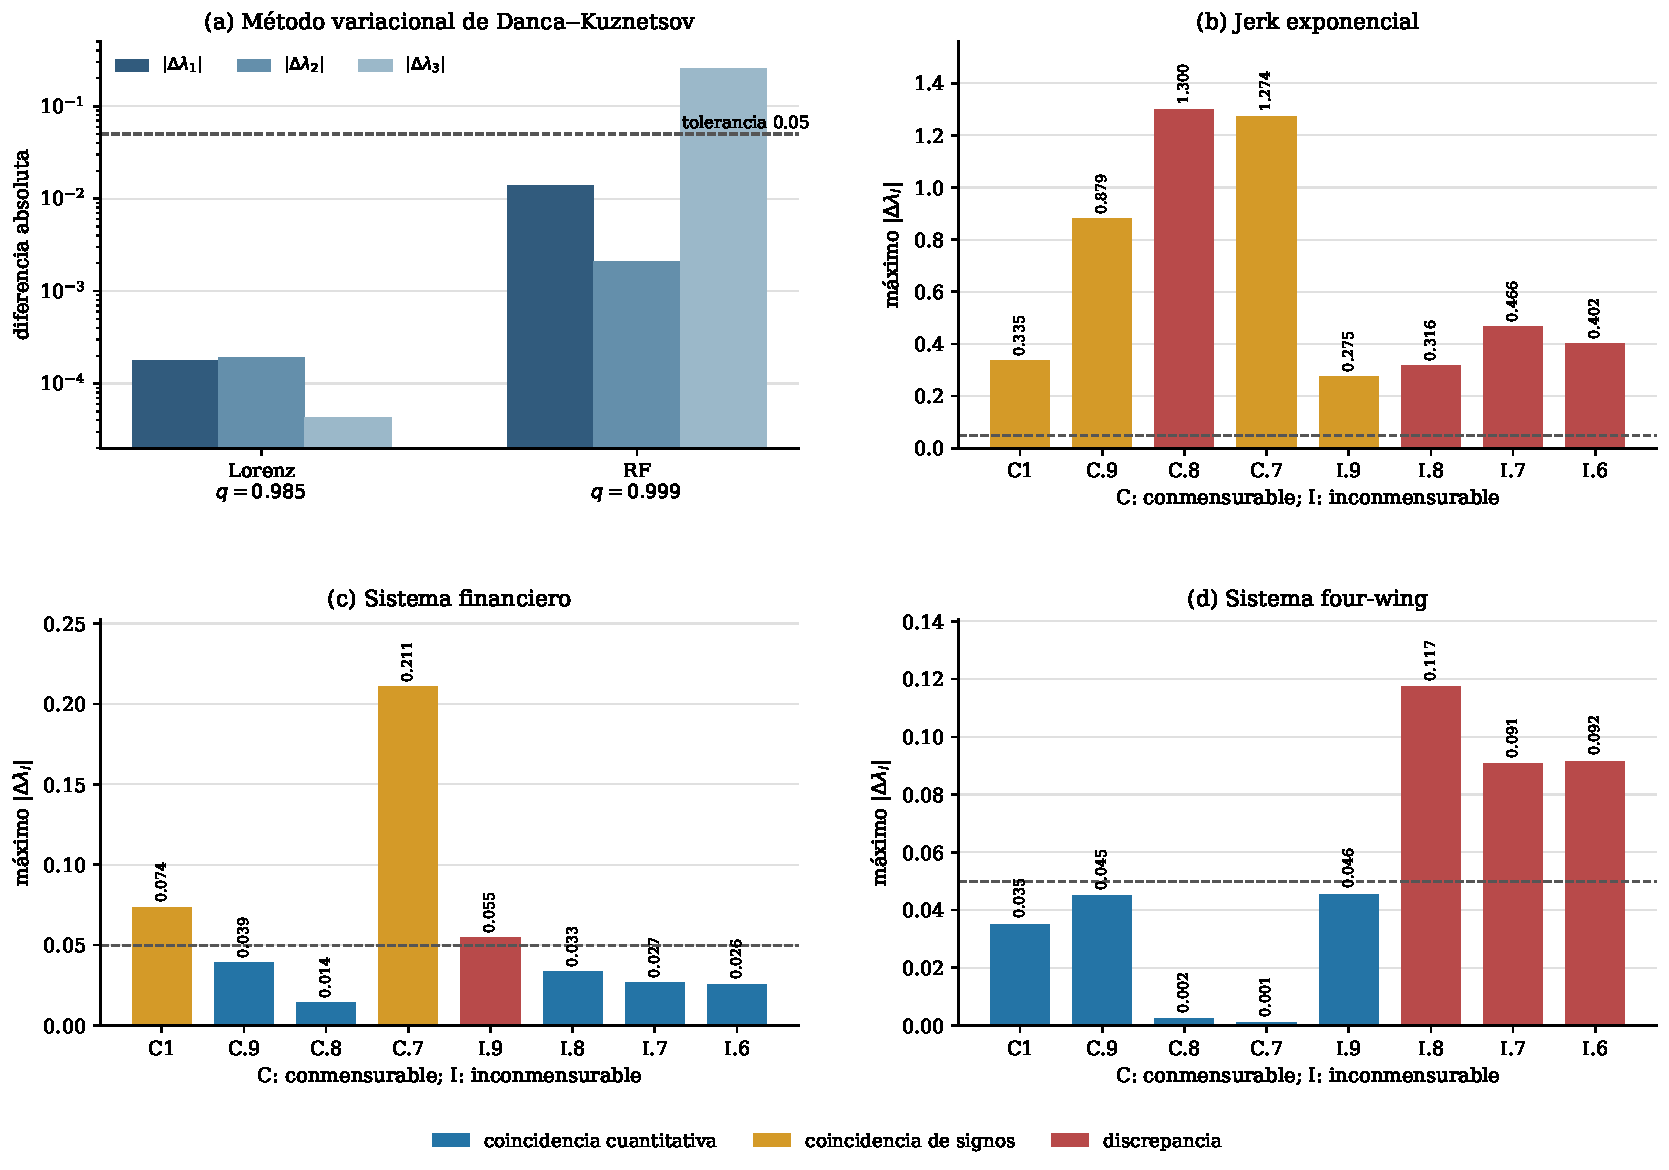
\includegraphics[width=0.96\linewidth]{figures/nonchua_benchmarks/lyapunov_validation_overview.pdf}
\caption{Comparación numérica de los exponentes publicados y calculados. El
panel DK2018 muestra los dos casos variacionales; los paneles Fischer resumen
el error máximo por fila y distinguen coincidencias cuantitativas, apoyo por
patrón de signos y discrepancias.}
\label{fig:nonchua-lyapunov-validation}
\end{hafocommonfigure}

\subsection{Alcance de las conclusiones dinámicas}

Los exponentes de Lorenz, RF, jerk, financiero y four-wing comparan métodos
de cálculo bajo configuraciones publicadas. La clasificación de ocultedad
requiere localizar un conjunto recurrente, comprobar su persistencia al
variar paso y método, y analizar vecindades de todos los equilibrios. La
continuación hasta el sistema objetivo se utiliza cuando la ruta de
localización la requiere; las semillas directas y los PP permiten otras
rutas. Estos cinco casos tienen diagnósticos de Lyapunov, pero carecen del
análisis de cuenca necesario para clasificarlos como ocultos. Kalman--Fitts,
MAVPD y PLL sí cuentan con conjuntos localizados y sondeos de vecindad,
dentro del alcance finito indicado en sus resultados.

\clearpage

\section{Comparación de los problemas de localización}

\begin{table}[ht]
\centering
\small
\caption{Comparación algebraica de los dos candidatos prioritarios.}
\begin{tabularx}{\linewidth}{>{\raggedright\arraybackslash}p{0.24\linewidth}XX}
\toprule
Propiedad & Lorenz generalizado & Rabinovich--Fabrikant\\
\midrule
Orden no lineal & cuadrático & cuadrático y cúbico\\
Canales elegidos & 3 & 5\\
Truncación inicial & \(H=2\) & \(H=3\)\\
Equilibrios & 3 & 5\\
Estables a \(q\) objetivo & \(E_+,E_-\) & \(E_1,E_2\)\\
Inestables a \(q\) objetivo & \(E_0\) & \(E_0,E_3,E_4\)\\
Simetría & \((x_1,x_2,x_3)\mapsto(-x_1,-x_2,x_3)\) & la misma\\
Riesgo algebraico & bajo--medio & medio--alto\\
Dificultad numérica & historia y cuenca & historia, términos cúbicos,
divergencia y transitorios\\
Dinámica del candidato & referencia bibliográfica & referencia bibliográfica\\
\bottomrule
\end{tabularx}
\end{table}

Lorenz generalizado requiere menos canales y una truncación inicial \(H=2\).
Su cota absorbente controla las trayectorias de reinicio y la cuenca
bibliográfica alrededor del único equilibrio inestable ofrece una referencia
para los sondeos. RF incorpora términos cúbicos, tres equilibrios inestables y
trayectorias divergentes; exige mayor resolución armónica y controles de escape.

\section{Identidades y estabilidad local}

Los parámetros racionales
\(r=34/5\), \(a_L=-1/2\), \(a_R=1/10\) y \(b_R=719/2500\) permiten
mantener exactas las identidades antes de evaluar las raíces numéricas.

\begin{longtable}{>{\raggedright\arraybackslash}p{0.34\linewidth}
>{\raggedright\arraybackslash}p{0.17\linewidth}
>{\raggedright\arraybackslash}p{0.40\linewidth}}
\caption{Identidades algebraicas y clasificación local.}\\
\toprule
Comprobación & Resultado & Evidencia\\
\midrule
\endfirsthead
\toprule
Comprobación & Resultado & Evidencia\\
\midrule
\endhead
Identidad Lur'e de Lorenz & \ok &
\(A_Lx+B_L\Phi_L(x)-F_L(x)=0\) en las tres componentes.\\
Transferencia de Lorenz & \ok &
Las nueve entradas del residuo simbólico son cero.\\
Equilibrios de Lorenz & \ok &
Residuo simbólico cero; máximo numérico \(1.07\times10^{-14}\).\\
Espectros de Lorenz & \ok &
Los valores propios satisfacen los polinomios característicos declarados; su
suma coincide con la traza de cada Jacobiano y los residuos numéricos son
inferiores a \(10^{-12}\).\\
Clasificación de Matignon de Lorenz & \ok &
\(E_0\) inestable; \(E_{\pm}\) estables a \(q=0.995\), margen \(0.0117288\).\\
Identidad Lur'e de RF & \ok &
\(A_Rx+B_R\Phi_R(x)-F_R(x)=0\) en las tres componentes.\\
Transferencia de RF & \ok &
Las quince entradas del residuo simbólico son cero.\\
Equilibrios RF & \ok &
Las dos ramas de~\eqref{nc:eq:rf-u} dan residuo simbólico cero; máximo numérico
\(1.06\times10^{-14}\).\\
Espectros y Matignon de RF & \ok &
Coinciden con la fuente al redondeo: \(E_{1,2}\) estables;
\(E_0,E_{3,4}\) inestables a \(q=0.998\).\\
\bottomrule
\end{longtable}

Estas identidades determinan la realización algebraica y la estabilidad
local. La localización del candidato requiere resolver el balance armónico,
integrar el PVI causal y estudiar su cuenca.

\section{Condiciones para la evaluación dinámica}

Las ecuaciones~\eqref{nc:eq:lorenz-hb-system} y
\eqref{nc:eq:rf-hb-system} definen los problemas multiharmónicos de generación
de semillas. Sus raíces numéricas requieren control del residual físico y
del truncamiento. Una semilla obtenida por esta ruta debe integrarse con
historia causal, continuarse cuando sea necesario y evaluarse con el campo
final fijo. La recurrencia, la robustez y los sondeos de todos los equilibrios
son problemas dinámicos independientes de las identidades algebraicas y de
los espectros locales.
